\documentclass[a4paper,14pt]{article}
\usepackage{float}
\usepackage{extsizes}
\usepackage{amsmath}
\usepackage{amssymb}
\everymath{\displaystyle}
\usepackage{geometry}
\usepackage{fancyhdr}
\usepackage{multicol}
\usepackage{graphicx}
\usepackage[brazil]{babel}
\usepackage[shortlabels]{enumitem}
\usepackage{cancel}
\columnsep=2cm
\hoffset=0cm
\textwidth=8cm
\setlength{\columnseprule}{.1pt}
\setlength{\columnsep}{2cm}
\renewcommand{\headrulewidth}{0pt}
\geometry{top=1in, bottom=1in, left=0.7in, right=0.5in}

\pagestyle{fancy}
\fancyhf{}
\fancyfoot[C]{\thepage}

\begin{document}
	
	\noindent\textbf{8FMA25~Matemática} 
	
	\begin{center}Revisão: área de um triângulo qualquer (Versão estudante)
	\end{center}
	
	\noindent\textbf{Nome:} \underline{\hspace{10cm}}
	\noindent\textbf{Data:} \underline{\hspace{4cm}}
	
	%\section*{Questões de Matemática}
    \begin{center}
    	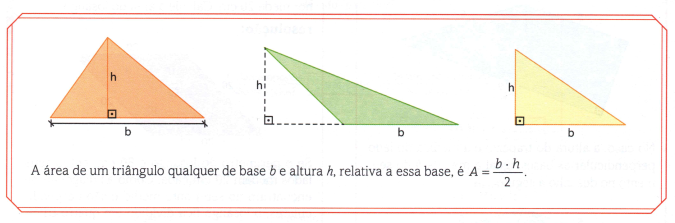
\includegraphics[width=1\linewidth]{8FMA25_imagens/imagem1}
    \end{center}
    
	\begin{multicols}{2}
		\begin{enumerate}
			\item Os lados do quadrado a seguir medem 8 cm. Ele foi quadriculado de 1 cm. A área da figura destacada é:
			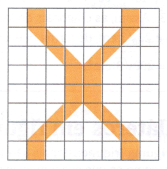
\includegraphics[width=1\linewidth]{8FMA25_imagens/imagem2}
			\begin{enumerate}
				\item 20 u.a.
				\item 16 u.a.
				\item 12 u.a.
				\item 9 u.a.
				\item 6 u.a.\\
			\end{enumerate}
		    \item Num triângulo isóceles, os lados medem 13 m e 6 m. Qual é a área do triângulo? \\\\\\\\\\\\\\\\\\\\\\\\\\\\\\\\\\\\\\\\
		    \item
		    \begin{enumerate}[a)]
		    	\item Considere o triângulo equilátero $ABC$ e $M$ e $N$ os pontos médios de $\overline{AB}$ e $\overline{AC}$, respectivamente. Se o segmento $MN$ tem medida igual a 6 cm, qual é a área do triângulo $ABC$? \\\\\\\\\\\\\\\\\\\\\\\\\\\\\\
		    	\item Considere o triângulo retângulo $ABC$ e $\overline{AH}$ sua altura relativa à hipotenusa $\overline{BC}$. Qual é a medida de $\overline{AC}$, se $BH = 6$ cm e $HC = 15$ cm? \\\\\\\\\\\\\\\\\\\\\\\\
		    \end{enumerate}
	        \item Calcule a área do quadrilátero a seguir, sabendo que o ângulo $\hat{A}$ é reto, o ângulo $\hat{C}$ mede $60^\circ$, $AB = 12$ cm e $BC = CD = 16$ cm.
	        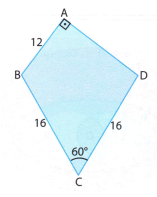
\includegraphics[width=1\linewidth]{8FMA25_imagens/imagem3}
	         \\\\\\\\\\\\\\\\\\\\\\\\\\\\\\\\\\\\\\\\\\
	        \item Determine os pontos $F$ e $G$ sobre a reta $CD$, de modo que as áreas do triângulo $AFG$ e do pentágono $ABCDE$ sejam iguais.\\
	        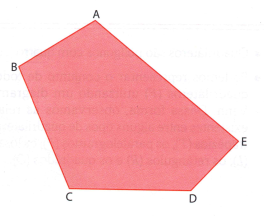
\includegraphics[width=1\linewidth]{8FMA25_imagens/imagem4}
	        \\\\\\\\\\\\\\\\\\\\\\\\\\\\\\\\\\\\\\\\\\\\\\\\\\
	        \item Calcule a área do triângulo a seguir:\\
	        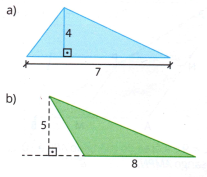
\includegraphics[width=1\linewidth]{8FMA25_imagens/imagem5}
	        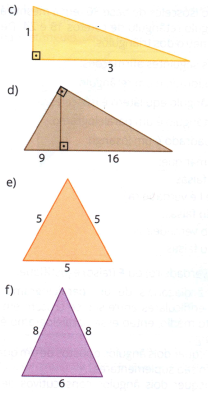
\includegraphics[width=1\linewidth]{8FMA25_imagens/imagem6}
	        \\\\\\\\\\\\
	        \item Um triângulo isóceles de área $9\sqrt{7}$ cm² tem altura relativa à sua base igual a $3\sqrt{7}$ cm. Qual é seu perímetro? \\\\\\\\\\\\\\\\\\\\
	        \item (Enem)~Para decorar a fachada de um edifício, um arquiteto projetou a colocação de vitrais compostos de quadrados de lado medindo 1 m, conforme a figura a seguir.\\
	        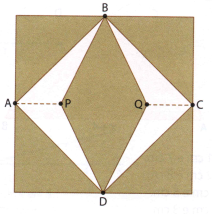
\includegraphics[width=1\linewidth]{8FMA25_imagens/imagem7}\\
	        Nesta figura, os pontos $A, B, C$ e $D$ são pontos médios dos lados do quadrado, e os segmentos $AP$ e $QC$ medem $\frac{1}{4}$ da medida do lado do quadrado. Para confeccionar um vitral, são usados dois tipos de materiais: Um para a parte colorida da figura, que custa R\$ 30,00 o m², e outro para a parte branca (regiões $ABPDA$ e $BCDQB$), que custa R\$ 50,00 o m².\\
	        De acordo com esses dados, qual é o custo dos materiais usados na fabricação de um vitral?
	        \begin{enumerate}[a)]
	        	\item R\$ 22,50
	        	\item R\$ 35,00
	        	\item R\$ 40,00
	        	\item R\$ 42,00
	        	\item R\$ 45,00
	        \end{enumerate}
            \item Um triângulo isóceles de base 36 tem a mesma área de um triângulo retângulo de catetos 18 a 24. Determine o perímetro dos triângulos.
		\end{enumerate}
	$~$ \\ $~$ \\ $~$ \\ $~$ \\ $~$ \\ $~$ \\ $~$ \\ $~$ \\ $~$ \\ $~$ \\ $~$ \\ $~$ \\ $~$ \\ $~$ \\ $~$ \\ $~$ \\ $~$ \\ $~$ \\ $~$ \\ $~$ \\ $~$
    \end{multicols}
\end{document}